% !TEX root = ./Vorlesungsmitschrift AGLA 2.tex  
\lecture{Fr 12.06. 10:15}{}
\subsection*{Zusammenhang Doppelverhältnis \( \leftrightarrow \) Teilverhältnis}
Seien \( p_0,p_1,p_2,p_3\in \projectionspaceover{1}{K} \) paarweise
verschieden und \( p_i=(1:\mu_i) \) für \( 0\leq i\leq 3 \) (wir schließen also hier den Punkt \( (0:1) \) aus). Dann gilt nach \thref{doppelverhaeltnis_berechnung}
\begin{align*}
  \doppelverhaeltnis{p_0}{p_1}{p_2}{p_3}&=\parens*{\braceannotate{\neq 0}{(\mu_0-\mu_2)}(\mu_1-\mu_3):(\mu_1-\mu_2)\braceannotate{\neq 0}{(\mu_0-\mu3)}}\\
  &=\parens*{\frac{\mu_1-\mu_3}{\mu_0-\mu_3}:\frac{\mu_1-\mu_2}{\mu_0-\mu_2}}\\
  &=(\teilverhaeltnis{\mu_3}{\mu_0}{\mu_1}:\teilverhaeltnis{\mu_2}{\mu_0}{\mu_1}).
\end{align*}
Also können wir in diesem Fall das Doppelverhältnis als \enquote{Verhältnis von Teilverhältnissen} verstehen.
\begin{bemerkungen*}
  Ist \( p_0=(0:1) \) und \( p_i=(1:\mu_i) \) für \( 1\leq i\leq 3 \) paarweise verschieden, so gilt nach \thref{doppelverhaeltnis_berechnung}
  \begin{align*}
    \doppelverhaeltnis{p_0}{p_1}{p_2}{p_3}&=(\mu_1-\mu_3:\mu_1-\mu_2)\\
    &=\parens*{\frac{\mu_3-\mu_1}{\mu_2-\mu_1}:1}\\
    &=(\teilverhaeltnis{\mu_1}{\mu_2}{\mu_3}:1).
  \end{align*}
\end{bemerkungen*}
\file{Desargues Pappos}
\subsection*{Zwei Anwendungen des Doppelverhältnisses}
\begin{satz}[Desargues]
  Sei \( \projectionspace{V} \) eine projektive Ebene und
  \begin{equation*}
    p_1,p_2,p_3,p_1',p_2',p_3' 
  \end{equation*}
  paarweise verschieden, sodass die Geraden
  \begin{equation*}
    p_1\vee p_1',p_2\vee p_2',p_3\vee p_3'
  \end{equation*}
  sich paarweise in einem gemeinsamen Punkt \( z \) schneiden.

  Dann sind die Schnittpunkte
  \begin{align*}
    a&\definedas (p_1\vee p_2)\cap (p_1'\vee p_2')\\
    b&\definedas (p_2\vee p_3)\cap (p_2'\vee p_3')\\
    c&\definedas (p_3\vee p_1)\cap (p_3'\vee p_1')
  \end{align*}
  in einer Geraden enthalten.
\end{satz}
\begin{proof}
  \begin{figure}
    \centering
    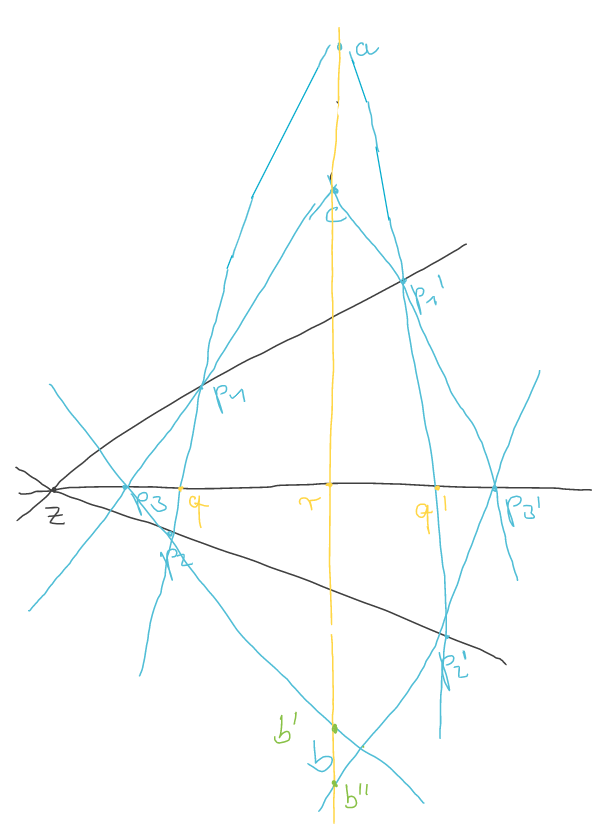
\includegraphics[width=0.9\linewidth]{desargues_visualisierung}
    \label{fig:desargues_visualisierung}
  \end{figure}
  Sei
  \begin{align*}
    q&\definedas (p_1\vee p_2)\cap (p_3\vee p_3')\\
    q'&\definedas (p_1\vee p_2')\cap (p_3\vee p_3')\\
    r&\definedas (a\vee c)\cap (p_3\vee p_3')\\
    b'&\definedas (a\vee c) \cap (p_2\vee p_3)\\
    b''&\definedas (a\vee c)\cap (p_2'\vee p_3')
  \end{align*}
  
  \begin{ziel*}
    Wir zeigen \( b'=b'' \), denn dann ist
    \begin{equation*}
      b'\cap b''\in (a\vee c)\cap \braceannotate{b}{(p_2\vee p_3)\cap (p_2'\vee p_3')}.
    \end{equation*}
  \end{ziel*}
  Die Punkte \( a\), \( c \) und \( r \), sind paarweise verschieden, es genügt also zu zeigen, dass
  \begin{equation*}
    \doppelverhaeltnis{a}{c}{r}{b'}=\doppelverhaeltnis{a}{c}{r}{b''}.
  \end{equation*}
  Betrachte die Zentralprojektion
  \begin{equation*}
    f_1\maps a\vee c\to a\vee p_1
  \end{equation*}
  mit Zentrum \( p_3 \). Es folgt 
  \begin{equation*}
    \doppelverhaeltnis{a}{c}{r}{b'}=\doppelverhaeltnis{a}{p_1}{q}{p_2}.
  \end{equation*}
  Verwende als Nächstes die Zentralprojektion
  \begin{equation*}
    f_2\maps a\vee p_1\to  a\vee p_1'
  \end{equation*}
  mit Zentrum \( z \) und erhalte
  \begin{equation*}
    \doppelverhaeltnis{a}{p_1}{q}{p_2}=\doppelverhaeltnis{a}{p_1'}{q'}{p_2'}
  \end{equation*}
  und danach die Zentralprojektion
  \begin{equation*}
    f_3\maps a\vee p_1'\to a\vee c
  \end{equation*}
  mit Zentrum \( p_3' \). Dann ist
  \begin{equation*}
    \doppelverhaeltnis{a}{p_1'}{q'}{p_2'}=\doppelverhaeltnis{a}{c}{r}{b''},
  \end{equation*}
  also
  \begin{equation*}
    \doppelverhaeltnis{a}{c}{r}{b'}=\doppelverhaeltnis{a}{c}{r}{b''}.
  \end{equation*}
\end{proof}
\begin{satz}[Pappos]
  Seien \( z,z'\subset \projectionspace{V} \) verschiedene Geraden in einer projektiven Ebene und
  \begin{equation*}
    p_1,p_2,p_3,p_1',p_2',p_3'
  \end{equation*}
  paarweise verschiedene Punkte mit
  \begin{align*}
    p_1,p_2,p_3&\in Z\\
    p_1',p_2',p_3'&\in Z'.
  \end{align*}
  Dann sind die Punkte
  \begin{align*}
    a&\definedas (p_1\vee p_2')\cap (p_1'\vee p_2)\\
    b&\definedas (p_2\vee p_3')\cap (p_2'\vee p_3)\\
    c&\definedas (p_3\vee p_1')\cap (p_3'\vee p_1)
  \end{align*}
  in einer Geraden enthalten.
\end{satz}
\begin{proof}
  \begin{figure}
    \centering
    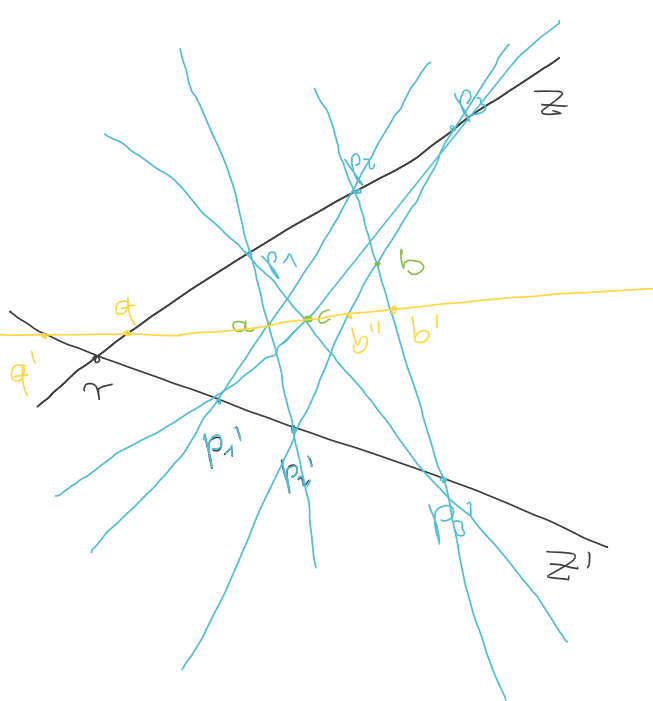
\includegraphics[width=\linewidth]{pappos_visualisierung}
    \label{fig:pappos_visualisierung}
  \end{figure}
  Wir definieren
  \begin{align*}
    r&\definedas Z\cap Z'\\
    q&\definedas (a\vee c)\cap Z\\
    q'&\definedas (a\vee c)\cap Z'\\
    b'&\definedas (a\vee c)\cap (p_2\vee p_3')\\
    b''&\definedas (a\vee c)\cap(p_2'\vee p_3).
  \end{align*}
  Falls 
  \begin{equation*}
    r\in \set{p_1,p_2,p_3,p_1',p_2',p_3'},
  \end{equation*}
  \zb \( r=p_1 \), dann sind \( a,b,c \) in der Geraden \( p_1'\vee b \) enthalten. Ebenso können wir 
  \begin{equation*}
    a\in \set{p_1,p_2,p_3,p_1',p_2',p_3'}
  \end{equation*}
  Wir nehmen also an
  \begin{equation*}
    a,r\not\in \set{p_1,p_2,p_3,p_1',p_2',p_3'}.
  \end{equation*}
  \begin{ziel*}
    Zeige, dass \( b'=b'' \).
  \end{ziel*}
  Wir verwenden Zentralprojektionen
  \begin{equation*}
    f_1\maps a\vee c\to \braceannotate{Z}{p_1\vee p_2}
  \end{equation*}
  mit Zentrum \( p_3' \),
  \begin{equation*}
    \doppelverhaeltnis{q}{c}{q'}{b'}=\doppelverhaeltnis{q}{p_1}{r}{p_2}.
  \end{equation*}
  Danach
  \begin{equation*}
    f_2\maps \braceannotate{Z}{p_1\vee p_2}\to Z'
  \end{equation*}
  mit Zentrum \( a \),
  \begin{equation*}
    \doppelverhaeltnis{q}{p_1}{r}{p_2}=\doppelverhaeltnis{q'}{p_2'}{r}{p_1'}.
  \end{equation*}
  Verwende dann die Zentralprojektion
  \begin{equation*}
    f_3\maps Z'\to a\vee c
  \end{equation*}
  mit Zentrum \( p_3 \),
  \begin{equation*}
    \doppelverhaeltnis{q'}{p_2'}{r}{p_1'}=\doppelverhaeltnis{q'}{b''}{q}{c}.
  \end{equation*}
  Nach Symmetrie gilt
  \begin{equation*}
    \doppelverhaeltnis{q'}{b''}{q}{c}=\doppelverhaeltnis{q}{c}{q'}{b''}
  \end{equation*}
  und damit \( b'=b'' \).
\end{proof}
\file{Hauptsatz projektive Geometrie}
\section{Hauptsatz der projektiven Geometrie}
Seien \( V,W \) \( K \)-Vektorräume und
\begin{equation*}
  f\maps \projectionspace{V}\to\projectionspace{W}
\end{equation*}
eine Projektivität. Ist \( Z\subseteq \projectionspace{V} \) eine projektive Gerade, so ist auch
\begin{equation*}
  f(Z)\subseteq \projectionspace{W}
\end{equation*}
eine projektive Gerade.

\begin{frage*}
  Welche bijektiven Abbildungen
  \begin{equation*}
    g\maps \projectionspace{V}\to \projectionspace{W}
  \end{equation*}
  haben die Eigenschaft, dass Geraden auf Geraden abgebildet werden?
\end{frage*}
\begin{definition*}
  Seien \( V,W \) \( K \)-Vektorräume und \( g\maps \projectionspace{V}\to \projectionspace{W} \) eine bijektive Abbildung, sodass \( \forall p,p'\in \projectionspace{V} \)
  \begin{equation*}
    f(p\vee p')\subseteq f(p)\vee f(p').
  \end{equation*}
  Dann nennen wir \( g \) Kollineation.
\end{definition*}
\begin{beispiel*}
  Sei \( K \) ein Körper mit Automorphismus \( \alpha \) und \( F\maps V\to W \) eine injektive   lineare Abbildung, \dh 
  \begin{align*}
    F(v+v')&=F(v)+F(v')\quad \forall v,v'\in V\\
    F(\lambda v)&=\alpha(\lambda)F(v)\quad \forall \lambda\in K\logicspace \forall v\in V.
  \end{align*}
  Dann induziert \( F \) eine Abbildung
  \begin{equation*}
    \begin{split}
      \projectionmap{F}\maps \projectionspace{V}\%to \projectionspace{W}\\
      \projectionspace{V}\ni K\cdot v&\mapsto K\cdot F(v)\quad v\in V\setminus\zeroset.
    \end{split}
  \end{equation*}
\end{beispiel*}

\begin{definition*}
  Seien \( V,W \) \( K \)-Vektorräume. Wir nennen eine Abbildung
  \begin{equation*}
    f\maps \projectionspace{V}\to \projectionspace{W}
  \end{equation*}
  \emph{semiprojektiv}, falls es eine injektive semilineare Abbildung \( F\maps V\to W \) gibt mit
  \begin{equation*}
    f=\projectionmap{F}.
  \end{equation*}
  Falls \( f \) außerdem bijektiv ist, so nennen wir \( f \) Semiprojektivität.
\end{definition*}
\begin{bemerkung*}
  Ist \( F\maps V\to W \) semilinear, so gilt
  \begin{equation*}
    F(K\cdot v)=K\cdot F(v),
  \end{equation*}
  dnn
  \begin{align*}
    F(K\cdot v)&=\Set{F(\lambda v)|\lambda\in K}\\
    &=\Set{\alpha(\lambda)F(v)|\lambda\in K}\\
    &\explain{\alpha \text{ ist bijekti}}{=}\Set{\lambda F(v)|\lambda\in K}\\
    &=K\cdot F(v).
  \end{align*}
\end{bemerkung*}
\begin{beispiel*}
  Betrachte den Körper
  \begin{equation*}
    \rationals(\sqrt{2})=\Set{a+b\sqrt{2}|a,b\in \rationals}
  \end{equation*}
  mit Automorphismus
  \begin{equation*}
    a+b\sqrt{2}\mapsto a-b\sqrt{2}\quad a,b\in \rationals.
  \end{equation*}
  Dann ist
  \begin{equation}
    \begin{split}
      F\maps \rationals(\sqrt{2})^3&\to \rationals(\sqrt{2})^3\\
      (a_1+b_1\sqrt{2},a_2+b_2\sqrt{2},a_3+b_3\sqrt{2})&\mapsto (a_1-b_1\sqrt{2}, a_2-b_2\sqrt{2},a_3-b_3\sqrt{2})
    \end{split}
  \end{equation}
  eine semilineare Abbildung, die eine Semiprojektivität
  \begin{equation*}
    \projectionmap{F}\maps \projectionspaceover{2}{\rationals(\sqrt{2})}\to\projectionspaceover{2}{\rationals(\sqrt{2})}
  \end{equation*}
  induziert.
\end{beispiel*}
\begin{frage*}
  Ist \( \projectionmap{F} \) eine Projektivität über \( \rationals(\sqrt{2}) \)?
\end{frage*}
\begin{lemma}
  Seien \( V,W \) \( K \)-Vektorräume, \( f\maps \projectionspace{V}\to \projectionspace{W} \) eine semiprojektive Abbildung und \( Z\subseteq \projectionspace{V} \) ein projektiver Unterraum. Dann ist \( f(Z)\subseteq \projectionspace{W} \) ein projektiver Unterraum mit 
  \begin{equation*}
    \projectivedim-{f(Z)}=\projectivedim-{Z}.
  \end{equation*}
\end{lemma}
\begin{proof}
  Sei \( Z=\projectionspace{U} \) mit \( U\untervektorraum V \) \( K \)-Untervektorraum,
  \begin{equation*}
    \dim-{U}=\projectivedim-{Z}+1=r.
  \end{equation*}
  Sei \( F\maps V\to W \) injektiv, semilinear zum Automorphismus \( \alpha \) und \( f=\projectionmap{F} \). Sei \( v_1,\dotsc,v_r\in V \) eine Basis von \( U \) als \( K \)-Vektorraum. Wir berechnen
  \begin{align*}
    F(U)&=F(K\cdot v_1+\dotsb+K v_r)\\
    &=\Set{F(\lambda_1 v_1+\dotsb+\lambda_r v_r)|\lambda_1,\dotsc,\lambda_r\in K}\\
    &\explain{F \text{ ist semilinear}}{=}\Set{\alpha(\lambda_1)F(v_1)+\dotsb+\alpha(\lambda_r)F(v_r)|\lambda_1,\dotsc,\lambda_r\in K}
    &=\Set{\lambda_1 F(v_1)+\dotsb+\lambda_r F(v_r)|\lambda_1,\dotsc,\lambda_r\in K}\\
    &=K\cdot F(v_1)+\dotsb+K\cdot F(v_r)
  \end{align*}
  ist \( K \)-Untervektorraum on \( W \). Es ist \( \dim-{F(U)}=r \), da \( F \) injektiv + semilinear ist. Verwende nun
  \begin{equation*}
    f(Z)=\projectionspace{F(U)}.
  \end{equation*}  
\end{proof}
\begin{satz}[Hauptsatz der projektiven Geometrie]\label{hauptsatz_projektive_geometrie}
  Seien \( V,W \) \( K \)-Vektorräume mit \( \dim-{V}=\dim-{W}\geq 3 \) und \( f\maps \projectionspace{V}\to\projectionspace{W} \) eine Kollineation. Dann ist \( f \) eine Semiprojektivität.
\end{satz}
\begin{bemerkung*}
  Im Fall \( K=\reals \) folgt sogar, dass \( f \) eine Projektivität ist, \dh für reelle projektive Räume der Dimension \( \geq 2 \) sind die Begriffe Kollineation und Projektivität gleichbedeutend.
\end{bemerkung*}